\subsection{Unleashing Precision: What Can a Vector Network Analyzer Measure?}

\begin{tcolorbox}[colback=gray!10, colframe=black, title=E4B11] 

Which of the following can be measured with a vector network analyzer? 

\begin{enumerate}[label=\Alph*)]
    \item Input impedance
    \item Output impedance
    \item Reflection coefficient
    \item \textbf{All these choices are correct}
\end{enumerate} \end{tcolorbox}

\subsubsection{Related Concepts}

A Vector Network Analyzer (VNA) is an essential tool in radio communication and electronics for measuring the electrical characteristics of components and systems. Understanding what a VNA can measure is crucial in designing and analyzing RF circuits. 

In regards to the options provided:

1. \textbf{Input Impedance (A)}: This refers to the impedance seen by the source connected to a device. It is significant in determining how much of the signal will be reflected back to the source versus transmitted through the device.

2. \textbf{Output Impedance (B)}: Similar to input impedance, it describes the impedance looking into the output of a device. Proper matching between output impedance and load impedance minimizes signal reflection.

3. \textbf{Reflection Coefficient (C)}: This parameter quantifies how much of the incident signal is reflected by a discontinuity in a transmission line. The reflection coefficient is derived from the input and output impedances and is critical in assessing how well a system is matched.

Since a VNA measures the aforementioned parameters, the correct answer to the question is \textbf{D: All these choices are correct}. The VNA essentially captures the relationship between input and output signals to deliver insights into impedance and reflection characteristics across a frequency range.

\subsubsection{Calculations}

In practice, to calculate the reflection coefficient ($\Gamma$), one can use the following formula:

\[
\Gamma = \frac{Z_L - Z_0}{Z_L + Z_0}
\]

where \(Z_L\) is the load impedance and \(Z_0\) is the characteristic impedance of the system. 

For example, if we have a load impedance \(Z_L = 50 \Omega\) and a characteristic impedance \(Z_0 = 75 \Omega\):

\[
\Gamma = \frac{50 \Omega - 75 \Omega}{50 \Omega + 75 \Omega} = \frac{-25 \Omega}{125 \Omega} = -0.2
\]

This negative value of the reflection coefficient indicates that some of the signal is being reflected back, and a more comprehensive analysis can be conducted using the VNA to understand the level of mismatch.

\subsubsection{Diagram}

Below is a simple schematic using TikZ to illustrate the connection of a VNA to a load.

\begin{center}
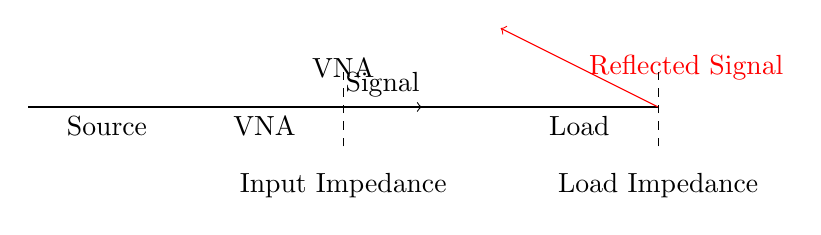
\begin{tikzpicture}
    % Components
    \draw (0,0) -- (2,0) node[midway, below] {Source} -- (4,0) node[midway, below] {VNA} -- (6,0) -- (8,0) node[midway, below] {Load};
    \node at (4,0.5) {VNA};
    \draw[->] (4,0) -- (5,0) node[midway, above] {Signal};

    % Reflections
    \draw[->, red] (8,0) -- (6,1) node[midway, right, red] {Reflected Signal};
    
    % Labels
    \draw[dashed] (4,-0.5) -- (4,0.5);
    \draw[dashed] (8,-0.5) -- (8,0.5);
    \node at (4,-1) {Input Impedance};
    \node at (8,-1) {Load Impedance};
\end{tikzpicture}
\end{center}
